\documentclass[12pt]{article}
\usepackage{tabularx} % Required for controlling table width
\usepackage{float}
\usepackage{graphicx} 
\usepackage[T1]{fontenc}
\begin{document}
\section{Arhitektura i dizajn sustava}

\begin{itemize}
	\item \textbf{Izbor arhitekture}
	      	      
	      Našom aplikacijom želimo olakšati organizaciju donacija krvi, samim
	      donatorima želimo omogućiti pristup donacijama, potvrdama i akcijama.
	      Zavodi bi trebali moći lako potvrđivati donacije, planirati nove akcije i pratiti
	      zalihe krvi.
	      	      
	      Kako bi pravilno izabrali arhitekturu projekta, izdvojili smo nekoliko
	      ciljeva:
	      \begin{itemize}
	      	\item Moderan dizajn sučelja i korisničko iskustvo:
	      	      	      	      
	      	      Sučelje aplikacije igra ključnu ulogu u privlačenju i zadržavanju korisnika.
	      	      Želimo moderan dizajn sučelja i intuitivnu navigaciju.
	      	      	      	      
	      	\item Brzina i pouzdanost:
	      	      	      	      
	      	      Korisnici očekuju da aplikacija radi brzo i pouzdano. To podrazumijeva
	      	      optimizaciju performansi, uključujući brzo učitavanje stranica i brze odgovore
	      	      na korisničke akcije.
	      	      	      	      
	      	\item Proširivost aplikacije:
	      	      	      	      
	      	      Planiranje za buduće proširenje aplikacije je ključno. To uključuje
	      	      dizajniranje arhitekture koja omogućava dodavanje novih značajki i
	      	      funkcionalnosti bez značajnih prepravki. Korištenje modularnog pristupa
	      	      i komponentne arhitekture može olakšati proširenje i održavanje aplikacije.
	      	      	      	      
	      	\item Lakoća održavanja i popravaka:
	      	      	      	      
	      	      Da bi se olakšao proces održavanja i ispravaka u aplikaciji, trebamo
	      	      pravilno organizirati i dokumentirati svoj kod. Pravilna dokumentacija
	      	      olakšava novim članovima tima da se brzo upuste u kod i razumiju njegovu
	      	      strukturu.
	      	      	      	      
	      	\item Rad više ljudi istovremeno:
	      	      	      	      
	      	      Ako planiramo da više ljudi radi na aplikaciji, važno je organizirati
	      	      razvojni proces na način koji omogućava suradnju i sprječava konflikte
	      	      u kodu. Verzioniranje koda i pravilna upotreba
	      	      grana omogućit će razvojnicima da rade neovisno i integriraju svoje
	      	      promjene bez problema.
	      \end{itemize}
	      	      
	      Uzimajući navedene ciljeve u obzir, kako bismo jasno razdvojili odgovornosti
	      i pojednostavili razvoj aplikacije, odlučili smo se za klijent-poslužitelj
	      arhitekturu u kombinaciji s odgovarajućom bazom podataka koristeći načela
	      objektno orijentiranog programiranja.
	      	      
	\item \textbf{Organizacija sustava}
	      	      
	      Klijentski sloj arhitekture omogućuje jednostavnu uporabu aplikacije donatorima.
	      Donatori će imati mogućnost pregledavati dostupne akcije za doniranje, brzo
	      se prijavljivati za sudjelovanje u akcijama, pregledavati svoju donatorsku
	      povijest te jednostavno dohvaćati potrebne potvrde i dokumente. Osim toga,
	      zavodi će također imati koristi od klijentskog dijela jer će im olakšati
	      proces potvrđivanja donacija i postavljanje novih akcija.
	      	      
	      Poslužiteljski sloj aplikacije je odgovoran za dohvat podataka iz baze i
	      slanje istih klijentskom sloju. Također, on će obavljati logičke operacije
	      kao što je uzimanje krvi s najstarijim datumom sa zalihe i slično.
	      	      
	      U sklopu baze podataka spremat ćemo ključne informacije o donacijama, potvrdama,
	      akcijama, zalihama krvi i drugim relevantnim podacima.
	      	      
	\item \textbf{Organizacija aplikacije}
	      	      
	      Za klijentski dio aplikacije odabrali smo React zbog niza prednosti koje pruža.
	      React je poznat po svojim impresivnim performansama, sposobnosti reagiranja
	      na promjene u stanju aplikacije, komponentnoj arhitekturi koja olakšava
	      razvoj i održavanje te ponovnoj upotrebljivosti komponenata, što odgovara objektno
	      orijentiranom načinu programiranja.
	      	      
	      Poslužiteljski dio naše aplikacije temelji se na Node.js-u i Express.js-u.
	      Ovaj izbor je napravljen s ciljem postizanja visoke učinkovitosti
	      izvođenja i jednostavnosti razvoja. Node.js je poznat po svojoj prilagodljivosti
	      i sposobnosti obrade velikog broja istovremenih korisnika, što ga čini
	      idealnim izborom za razvoj aplikacije ovog tipa.
	      	      
	      Za olakšavanje komunikacije s bazom podataka, odlučili smo se koristiti Sequelize,
	      ORM alatom koji omogućava jednostavno modeliranje i pristup podacima. Sequelize
	      nam omogućava definiranje modela koji se preslikavaju u tablice baze podataka.
	      Također, možemo koristiti seed skripte za jednostavno popunjavanje tablica
	      podacima za svrhe testiranja aplikacije. Za bazu podataka odabrali smo
	      PostgreSQL zbog njegove pouzdanosti i kompatibilnosti sa Sequelize-om.
	      
	      \begin{figure}[H]
	      	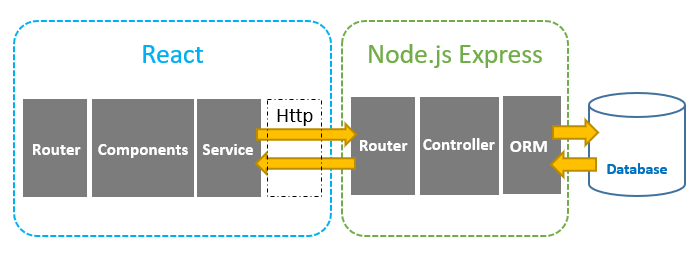
\includegraphics[scale=0.6]{slike/ArchitectureDiagram.png} 
	      	\centering
	      	\caption{Slojevi arhitekture}
	      	\label{fig:sa}
	      \end{figure}
	      
	      I klijentski i poslužiteljski dio naše aplikacije koriste MVC (Model-View-Controller) arhitekturni obrazac:
	      
	      Klijentski dio dohvaća podatke putem API poziva poslužitelju te ih pohranjuje unutar React komponenata, što predstavlja modelni dio arhitekture. Nadalje, komponente su odgovorne za iscrtavanje korisničkog sučelja, što predstavlja view dio arhitekture. Kontroler u klijentskom dijelu predstavljaju React komponente koje upravljaju stanjem aplikacije i komunikacijom s poslužiteljem.
	      
	      Poslužiteljski dio koristi ORM tehnologiju kako bi dohvatio i spremio podatke u bazu, što predstavlja modelni dio arhitekture. View dio poslužiteljskog dijela obuhvaća pripremu podataka za slanje klijentu, dok kontroleri obrađuju HTTP zahtjeve i vraćaju odgovore klijentskom dijelu. S ovakvim pristupom postižemo jasnu i efikasnu organizaciju aplikacije.
	      
	      \begin{figure}[H]
	      	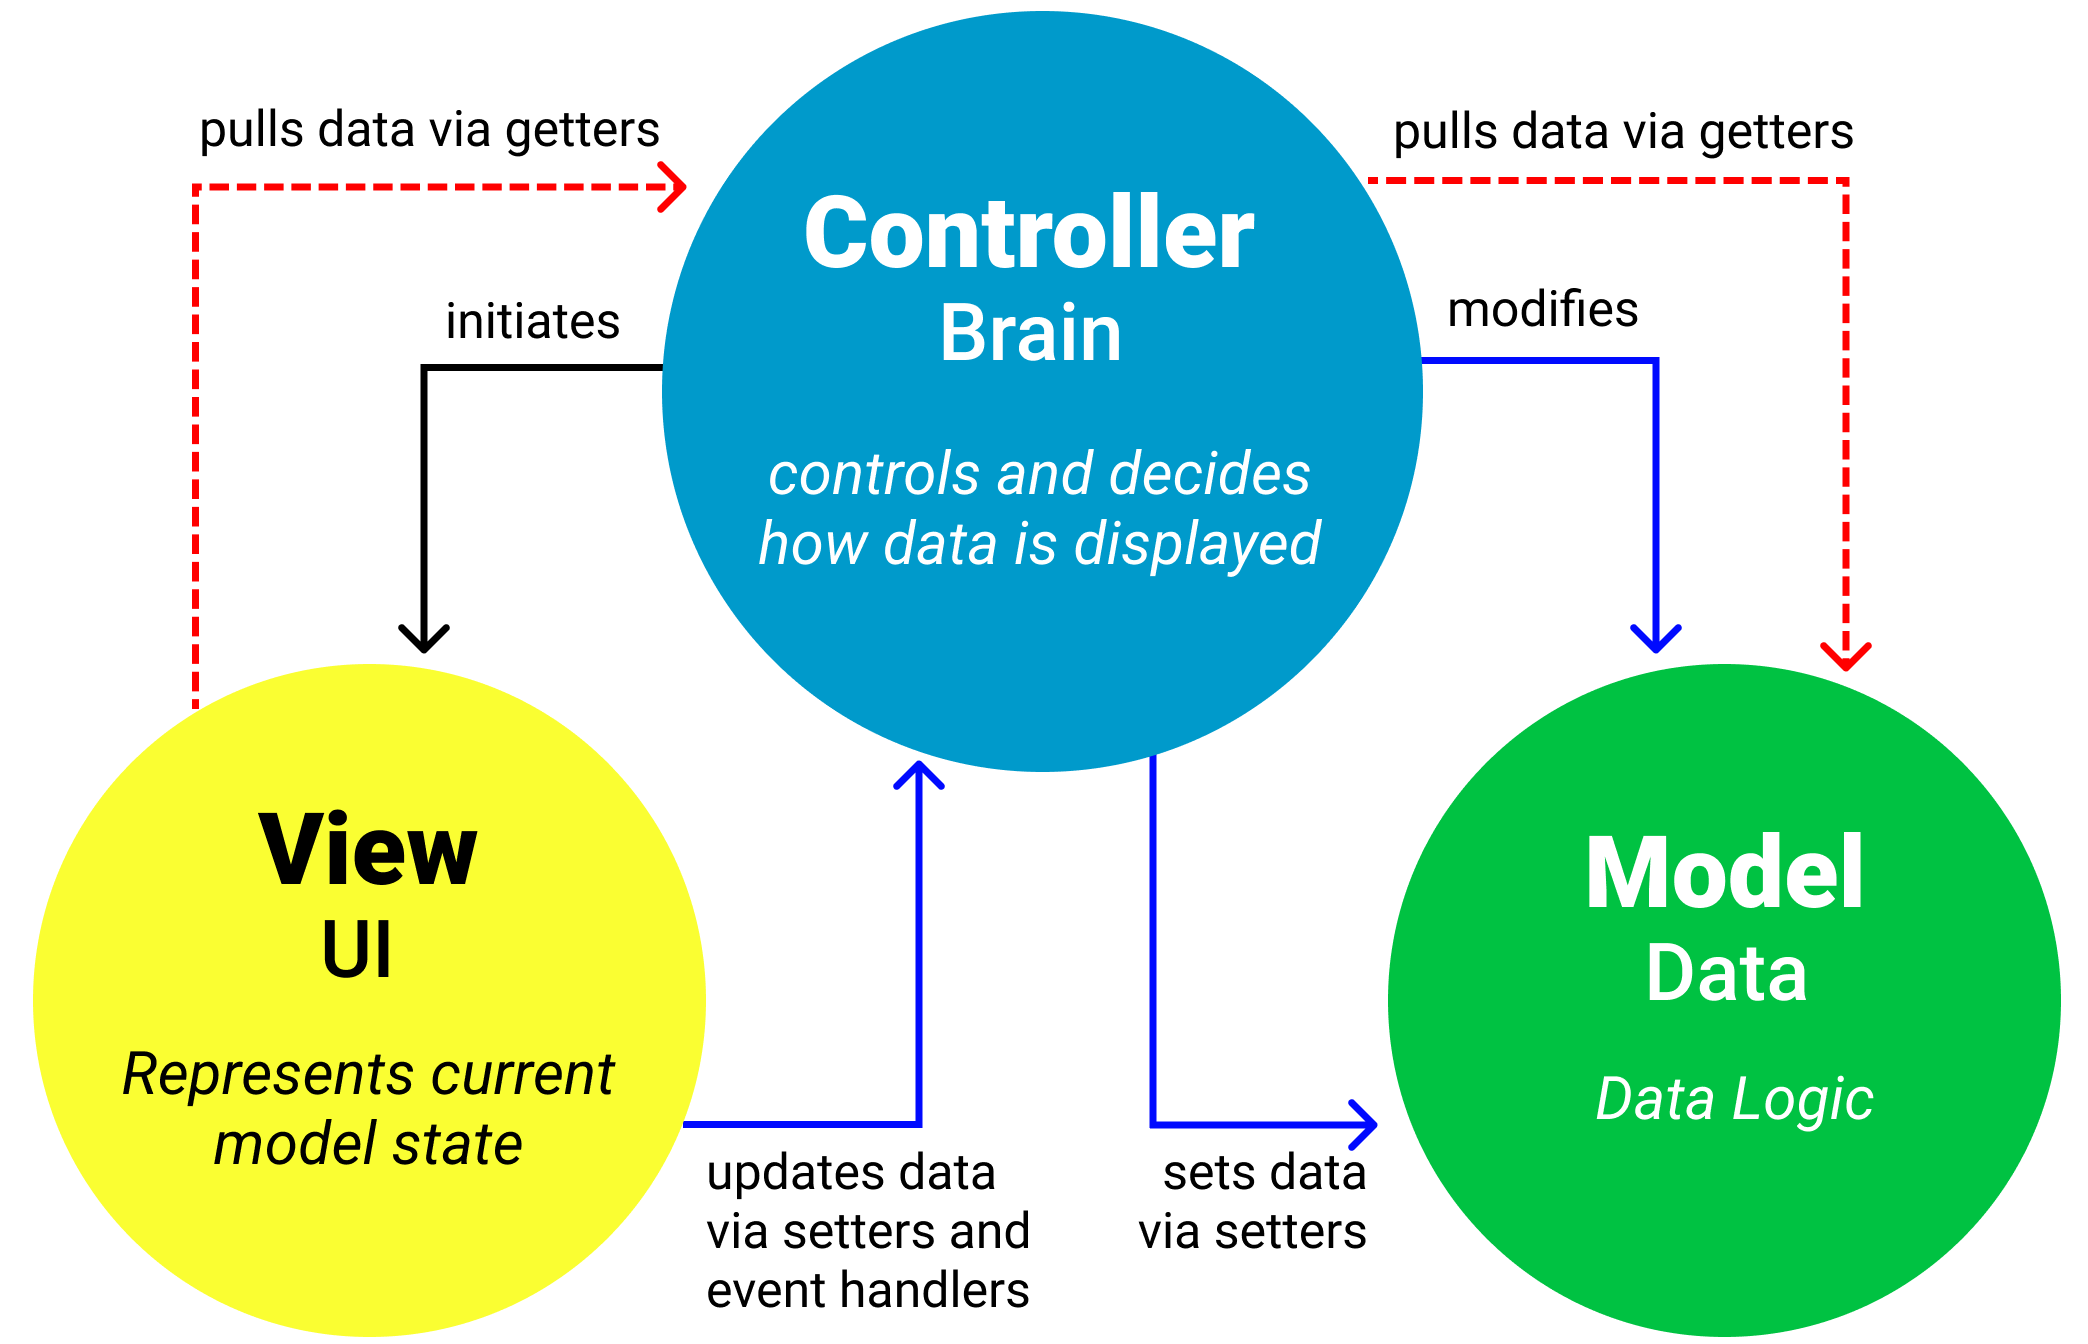
\includegraphics[scale=0.15]{slike/MVC.png}
	      	\centering
	      	\caption{MVC stil arhitekture}
	      	\label{fig:mvc}
	      \end{figure}
	      
	      
\end{itemize}

\subsection{Baza podataka}

Za trajnu pohranu podataka odlučili smo koristiti relacijsku bazu podataka i sustav PostgreSQL. Relacijske baze podataka su vrsta baza podataka koje koriste relacijski model za organizaciju i upravljanje podacima. Relacijski model podrazumijeva da se podaci pohranjuju u tablicama s redcima i stupcima, gdje su podaci organizirani u relacijama. Ovo omogućava efikasno upravljanje, pohranu i pretraživanje podataka, te osigurava konzistentnost i integritet podataka. PostgreSQL je snažan i popularan open-source sustav za upravljanje relacijskim bazama podataka. 

Baza podataka naše aplikacije sastoji se od sljedećih tablica:

\begin{itemize}
	\item  Donors
	\item  Donations
	\item  Certificates
	\item  BloodBanks
	\item  Actions
	\item  ActionRegistrations
\end{itemize}

\clearpage % Start a new page
\subsubsection{Opis tablica}

\noindent
\textbf{Donors (Donatori)} tablica pohranjuje informacije o donatorima, uključujući
njihovo ime, email adresu, lozinku, krvnu grupu, povezani institut za transfuziju,
broj donacija te datume stvaranja i ažuriranja zapisa. Ovaj entitet je u vezi \textit{One-to-Many}
s \textbf{Donations} preko \textit{id}, {Many-to-One} s \textbf{BloodBanks}
preko \textit{transfusionInstitute}, \textit{One-to-Many} s \textbf{Certificates}
preko \textit{id} i \textit{One-to-Many} s \textbf{ActionRegistrations} preko \textit{id}.
\begin{table}[H]
	\renewcommand{\arraystretch}{2}
	\centering
	\begin{tabularx}
		{1\textwidth}{|c|c|X|} \hline \textbf{Naziv Stupca} & \textbf{Vrsta
		podatka} & \textbf{Opis}    \\ \hline \cellcolor{LightGreen} id & INTEGER &
		Automatski povećavajući broj \\ \hline name & STRING & Ime donatora \\
		\hline email & STRING & Email donatora \\ \hline password & STRING
		         & Lozinka donatora \\ \hline bloodType & STRING & Krvna grupa donatora \\
		\hline \cellcolor{LightBlue} transfusionInstitute & STRING & Institut za transfuziju
		zadužen za donatora \\ \hline numberOfDonations & INTEGER & Broj donacija donatora
		\\ \hline createdAt & TIMESTAMP & Datum i vrijeme stvaranja zapisa \\ \hline
		updatedAt & TIMESTAMP & Datum i vrijeme posljednjeg ažuriranja zapisa \\ \hline
	\end{tabularx}
	\caption{Donors}
	\label{tab:my_label}
\end{table}
\clearpage % Start a new page

\noindent
\textbf{Donations (Donacije)} tablica sadrži informacije o donacijama, uključujući
datum donacije, adresu, upozorenje te podatke o povezanom donatoru. Također, sadrži
datume stvaranja i ažuriranja zapisa. Ovaj entitet je u vezi \textit{Many-to-One}
s \textbf{Donors} preko \textit{donorId}.
\begin{table}[H]
	\renewcommand{\arraystretch}{2}
	\centering
	\begin{tabularx}
		{1\textwidth}{|c|c|X|} \hline \textbf{Naziv Stupca} & \textbf{Vrsta
		podatka} & \textbf{Opis} \\ \hline \cellcolor{LightGreen}id & INTEGER & Automatski
		povećavajući broj \\ \hline date & DATE & Datum donacije \\ \hline address
		  & STRING & Adresa donacije \\ \hline warning & STRING & Upozorenje ako krv
		nije bila potpuno zdrava \\ \hline createdAt & TIMESTAMP & Datum i vrijeme
		stvaranja zapisa \\ \hline updatedAt & TIMESTAMP & Datum i vrijeme posljednjeg
		ažuriranja zapisa \\ \hline \cellcolor{LightBlue} donorId & INTEGER & ID
		donatora \\ \hline
		used & BOOLEAN & True ako je krv iskorištena, False ako je na zalihi\\ \hline
	\end{tabularx}
	\caption{Donations}
	\label{tab:my_label}
\end{table}
\clearpage % Start a new page

\noindent
\textbf{Certificates (Certifikati)} tablica pohranjuje informacije o certifikatima
koje donatori mogu postići. Uključuje naziv certifikata, njegove pogodnosti,
broj donacija potreban za certifikat te datume stvaranja i ažuriranja zapisa. Također,
sadrži podatke o povezanom donatoru. Ovaj entitet je u vezi \textit{Many-to-One}
s \textbf{Donors} preko \textit{donorId}.
\begin{table}[H]
	\renewcommand{\arraystretch}{2}
	\centering
	\begin{tabularx}
		{1\textwidth}{|c|c|X|} \hline \textbf{Naziv Stupca} & \textbf{Vrsta
		podatka} & \textbf{Opis} \\ \hline \cellcolor{LightGreen} id & INTEGER &
		Automatski povećavajući broj \\ \hline name & STRING & Naziv certifikata
		\\ \hline benefits & STRING & Pogodnosti certifikata \\ \hline
		numberOfDonations & INTEGER & Broj donacija potreban za certifikat \\
		\hline createdAt & TIMESTAMP & Datum i vrijeme stvaranja zapisa \\ \hline
		updatedAt & TIMESTAMP & Datum i vrijeme posljednjeg ažuriranja zapisa \\
		\hline \cellcolor{LightBlue} donorId & INTEGER & ID donatora \\ \hline
	\end{tabularx}
	\caption{Certificates}
	\label{tab:my_label}
\end{table}
\clearpage % Start a new page

\noindent
\textbf{BloodBanks (Zavodi za Transfuziju)} tablica pohranjuje informacije o
zavodima za transfuziju krvi, uključujući naziv zavoda za transfuziju, adresu,
broj donatora povezanih s zavodom za transfuziju te datume stvaranja i ažuriranja
zapisa. Ovaj entitet je u vezi \textit{One-to-Many} s \textbf{Donors} preko
\textit{id}.
\begin{table}[H]
	\renewcommand{\arraystretch}{2}
	\centering
	\begin{tabularx}
		{1\textwidth}{|c|c|X|} \hline \textbf{Naziv Stupca} & \textbf{Vrsta
		podatka} & \textbf{Opis} \\ \hline \cellcolor{LightGreen} id & INTEGER &
		Automatski povećavajući broj \\ \hline name & STRING & Naziv zavoda \\
		\hline email & STRING & Email adresa zavoda \\ \hline password & STRING &
		Lozinka zavoda \\ \hline address & STRING & Adresa zavoda \\ \hline
		numberOfDonors & INTEGER & Broj donatora povezan sa zavodom \\ \hline
		createdAt & TIMESTAMP & Datum i vrijeme stvaranja zapisa \\ \hline
		updatedAt & TIMESTAMP & Datum i vrijeme posljednjeg ažuriranja zapisa \\
		\hline
	\end{tabularx}
	\caption{BloodBanks}
	\label{tab:my_label}
\end{table}
\clearpage % Start a new page

\noindent
\textbf{Actions (Akcije)} tablica pohranjuje informacije o akcijama koje uključuju
adresu, datum, minimalni broj donatora potreban za akciju te datume stvaranja i
ažuriranja zapisa. Također, sadrži podatak o povezanom zavodu. Ovaj entitet je
u vezi \textit{Many-to-One} s \textbf{BloodBanks} preko \textit{bloodBankId}.
\begin{table}[H]
	\renewcommand{\arraystretch}{2}
	\centering
	\begin{tabularx}
		{1\textwidth}{|c|c|X|} \hline \textbf{Naziv Stupca} & \textbf{Vrsta
		podatka} & \textbf{Opis} \\ \hline \cellcolor{LightGreen}id & INTEGER & Automatski
		povećavajući broj \\ \hline address & STRING & Adresa akcije \\ \hline date
		  & DATE & Datum akcije \\ \hline minNumberOfDonors & INTEGER & Minimalni broj
		donatora potreban za akciju \\ \hline createdAt & TIMESTAMP & Datum i vrijeme
		stvaranja zapisa \\ \hline updatedAt & TIMESTAMP & Datum i vrijeme posljednjeg
		ažuriranja zapisa \\ \hline \cellcolor{LightBlue} bloodBankId & INTEGER &
		ID zavoda \\ \hline
	\end{tabularx}
	\caption{Actions}
	\label{tab:my_label}
\end{table}
\clearpage % Start a new page

\noindent
\textbf{ActionRegistrations (Registracije za Akcije)} tablica sadrži informacije
o registracijama za akcije. Uključuje ID akcije, ID donatora te datume stvaranja
i ažuriranja zapisa. Ovaj entitet je u vezi \textit{Many-to-One} s \textbf{Actions}
preko \textit{actionId} i \textit{Many-to-One} s \textbf{Donors} preko \textit{donorId}.
\begin{table}[H]
	\renewcommand{\arraystretch}{2}
	\centering
	\begin{tabularx}
		{1\textwidth}{|c|c|X|} \hline \textbf{Naziv Stupca} & \textbf{Vrsta
		podatka} & \textbf{Opis} \\ \hline \cellcolor{LightGreen} id & INTEGER &
		Automatski povećavajući broj \\ \hline \cellcolor{LightBlue} actionId & INTEGER
		         & ID akcije     \\ \hline \cellcolor{LightGreen}donorId & INTEGER & ID donatora
		\\ \hline createdAt & TIMESTAMP & Datum i vrijeme stvaranja zapisa \\ \hline
		updatedAt & TIMESTAMP & Datum i vrijeme posljednjeg ažuriranja zapisa \\ \hline
	\end{tabularx}
	\caption{ActionRegistrations}
	\label{tab:my_label}
\end{table}
\subsubsection{Dijagram baze podataka}
\begin{figure}[H]
	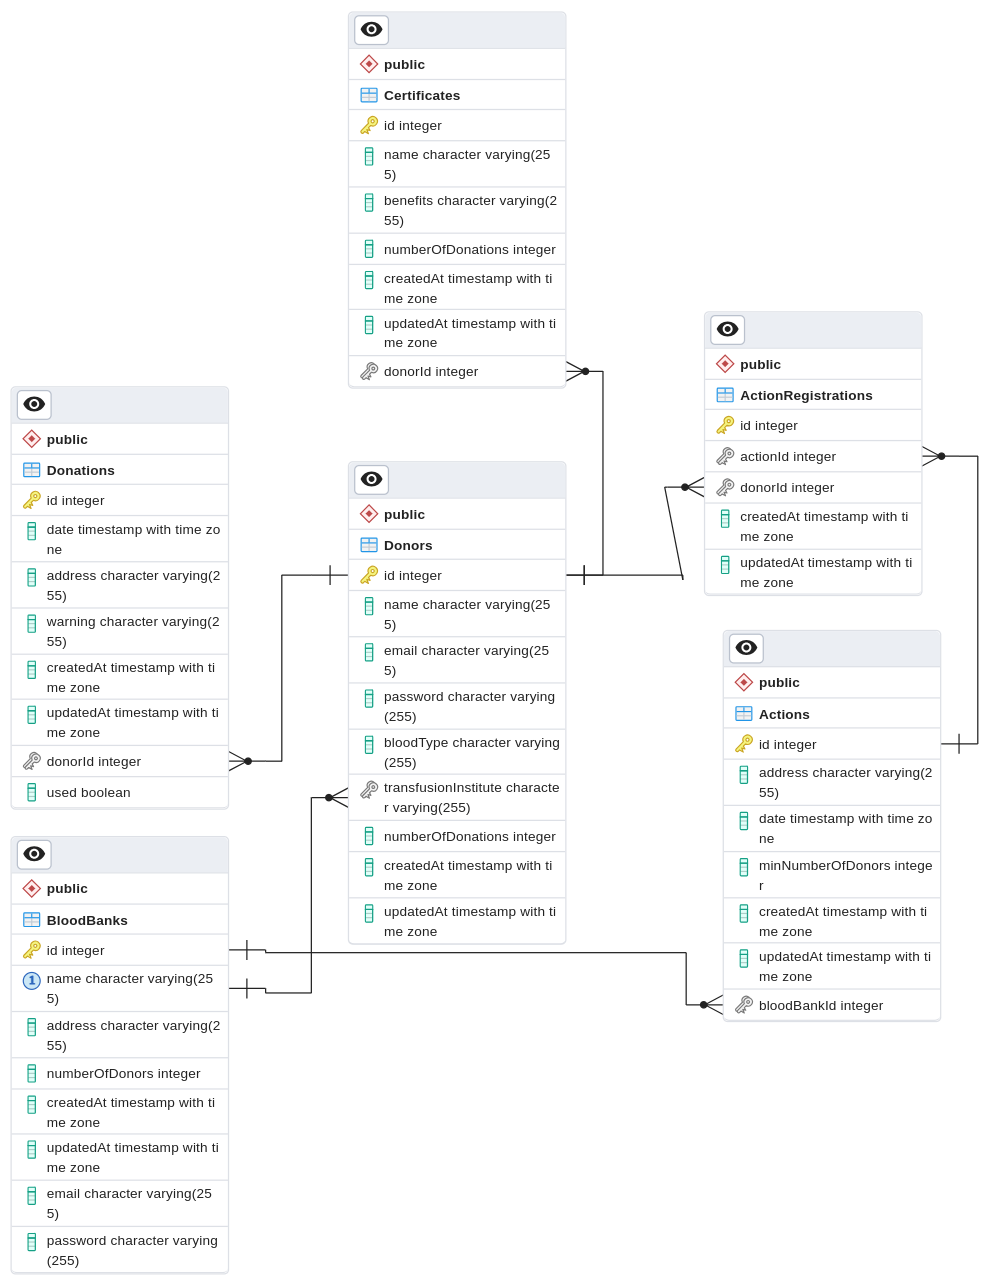
\includegraphics[scale=0.45]{slike/BazaERD.png}
	\centering
\end{figure}
\eject

\section{Dijagram razreda}

\textit{Potrebno je priložiti dijagram razreda s pripadajućim opisom. Zbog preglednosti
	je moguće dijagram razlomiti na više njih, ali moraju biti grupirani prema
	sličnim razinama apstrakcije i srodnim funkcionalnostima.}\\

\textbf{\textit{dio 1. revizije}}\\

\textit{Prilikom prve predaje projekta, potrebno je priložiti potpuno razrađen
	dijagram razreda vezan uz \textbf{generičku funkcionalnost} sustava. Ostale funkcionalnosti
	trebaju biti idejno razrađene u dijagramu sa sljedećim komponentama: nazivi
	razreda, nazivi metoda i vrste pristupa metodama (npr. javni, zaštićeni),
	nazivi atributa razreda, veze i odnosi između razreda.}\\

\textbf{\textit{dio 2. revizije}}\\

\textit{Prilikom druge predaje projekta dijagram razreda i opisi moraju
odgovarati stvarnom stanju implementacije}

\eject

\section{Dijagram stanja}

\textbf{\textit{dio 2. revizije}}\\

\textit{Potrebno je priložiti dijagram stanja i opisati ga. Dovoljan je jedan dijagram
	stanja koji prikazuje \textbf{značajan dio funkcionalnosti} sustava. Na primjer,
	stanja korisničkog sučelja i tijek korištenja neke ključne funkcionalnosti
jesu značajan dio sustava, a registracija i prijava nisu. }

\eject

\section{Dijagram aktivnosti}

\textbf{\textit{dio 2. revizije}}\\

\textit{Potrebno je priložiti dijagram aktivnosti s pripadajućim opisom. Dijagram
aktivnosti treba prikazivati značajan dio sustava.}

\eject
\section{Dijagram komponenti}

\textbf{\textit{dio 2. revizije}}\\

\textit{Potrebno je priložiti dijagram komponenti s pripadajućim opisom. Dijagram
komponenti treba prikazivati strukturu cijele aplikacije.}
\end{document}